\documentclass[border=0pt]{standalone}
\usepackage{graphicx}
\usepackage{fancyvrb}
\usepackage{xcolor}
\usepackage{bm}
\usepackage{pgf}
\usepackage{tikz}
\usetikzlibrary{automata, positioning, arrows}


\begin{document}

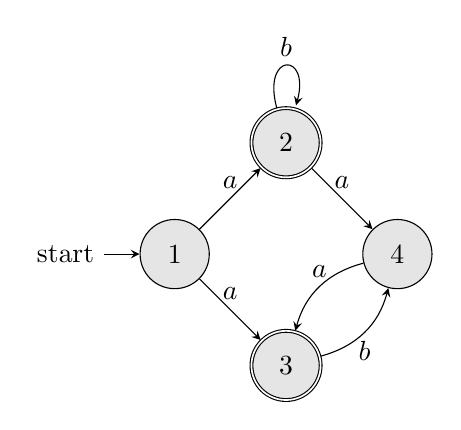
\begin{tikzpicture}[>=stealth,auto,node distance=20mm,state/.append style={fill=black!10}]
  \node[state, initial] (1) {$1$};
  \node[state, accepting, above right of=1] (2) {$2$};
  % \node[state, accepting, right of=2] (3) {$3$};
  \node[state, accepting, below right of=1] (3) {$3$};
  \node[state, above right of=3] (4) {$4$};

  \draw (1) edge[->,above] node {$a$} (2)
        (2) edge[loop above] node {$b$} (2)
        (1) edge[->,above] node {$a$} (3)
        (3) edge[->, below, bend right] node {$b$} (4)
        (4) edge[->, above, bend right] node {$a$} (3)
        (2) edge[->, above] node {$a$} (4);
\end{tikzpicture}
\end{document}
